\documentclass[article]{aaltoseries}
\usepackage[utf8]{inputenc}


\begin{document}
 
%=========================================================

\title{Implementing a Virtual Private Network System among Containers}

\author{Songlin Jiang% Your first and last name: do _not_ add your student number
\\\textnormal{\texttt{songlin.jiang@aalto.fi}}} % Your Aalto e-mail address

\affiliation{\textbf{Tutor}: Tuomas Aura} % First and last name of your tutor

\maketitle

%==========================================================

\begin{abstract}
This paper investigates the method of implementing a Virtual Private Network (VPN) system among containers. We implement a testing environment for two types of VPN, site-to-site and gateway-to-gateway, using both Vagrant with VirtualBox as the provider and Docker Compose to realize the same functionality. The result shows that, by migrating the test from the VMs to the Docker containers, we can save nearly 90\% of time and 94\% of memory used for testing the VPN systems. At the same time, the host machine still has no security risk increase.

\vspace{3mm}
\noindent KEYWORDS: Container, Network, Cloud, VPN

\end{abstract}


%============================================================


\section{Introduction}

In recent years, as an increasing number of applications have been moved to the cloud, container technologies such as Docker have received much attention from the industry and the academia. Containers are much more efficient and lightweight than virtual machines because containers share the Linux Kernel with the host. In contrast, virtual machines employ hardware virtualization and have their own instance of kernel, which needs more resources \cite{10.1145/2988336.2988337}.

VPNs are typically used in complex networking environments with many different network components. It is still a common practice \cite{9151942} to build and test network systems using virtual machines, which can be slow and troublesome. The problems can worsen when testing VPN systems, as each network component needs a virtual machine instance. It can be memory-consuming to simultaneously run multiple virtual machine instances on one host machine to simulate the network environment, which significantly perplexes testers with low-end devices and Continuous Integration / Continuous Delivery (CI/CD), as these environments are usually low on memory. Moreover, as Mac M1 / M2 chips are based on arm64 architecture, open-source virtual machine hypervisors are not currently well supported for arm64 hardware virtualization. However, arm64 is well supported by the containers \cite{9852232}.

Due to little research on implementing network systems using containers, this paper investigates the possibilities of implementing a VPN system based on Docker containers to overcome the disadvantages of virtual machines as mentioned above. This paper also analyze the functional and security limitations when implemented in this way.

This paper is organized as follows. Section 2 reviews the background of current technologies used for container networking. Section 3 defines our goal for implementing the VPN system using Docker containers, while Section 4 explains the details of our implementation. Section 5 presents our evaluation result by comparing the VPN system performance between the one implemented in the virtual machine and the one in the container. Finally, Section 6 provides the concluding remarks.

%============================================================


\section{Docker Networking System}
This section discusses the choice of the Docker container network driver for implementing the VPN system. It will also discuss how to enable routing and firewalls inside a container.

\subsection{Network Drivers}
Docker employs a pluggable networking subsystem. Several drivers can provide the docker network functionality, and the default ones include bridge, host, overlay, IPVLAN, MacVLAN, and none. We can choose one of them to implement the VPN system.

None, host, overlay drivers do not cater for our needs. Firstly, none driver disables all networking. Secondly, host driver is not necessary, as it can cause security implications due to its nature of sharing the same network stack with the host machine. In addition, overlay is not an appropriate option, as we are simulating the network system only on one host machine.

As a result, our possible candidates are bridge, IPVLAN, and MacVLAN. When looking into the details, bridge learns MAC addresses by looking into the frames headers of the communicating hosts. At the same time, the MacVLAN is a trivial bridge that does not need to learn as it already knows every MAC address it can receive \cite{9620212}. IPVLAN is very similar to MacVLAN, except that MacVLAN assigns a different MAC address to each attached docker container. In contrast, IPVLAN assigns the same MAC address to all containers attached to it \cite{7502883}.

MacVLAN is the best choice for our needs. As we will only use the driver to implement the internal network, there is no need to use advanced flood control and forwarding database manipulation that are specific to the bridge driver. Moreover, according to Docker's documentation related to networking \cite{docker_documentation_2023}, MacVLAN networks are the best choice when migrating from a VM setup, as MacVLAN makes the container appear as a physical device with its own MAC address. Besides, Gundall et al. \cite{9442123} conducts benchmarks for different virtualization technologies for networking overhead. The result shows that the MacVLAN driver has the best throughput while requiring the least CPU resources compared to other network drivers.

\subsection{Routing and Firewall}

Docker containers do not allow manipulating container network devices and setting routing tables or firewalls inside containers by default unless the net\_admin capability is assigned to the container.

According to capabilities man page \cite{capabilities}, assigning the net\_admin capability to containers allows performing the following network-related operations:
\begin{enumerate}
\setlength{\itemsep}{0pt}
\setlength{\parsep}{0pt}
\setlength{\parskip}{0pt}
\item Interface configuration;
\item Administration of IP firewall, masquerading, and accounting;
\item Modify routing tables;
\item Bind to any address for transparent proxying;
\item Set type-of-service (TOS);
\item Clear driver statistics;
\item Set promiscuous mode;
\item Enabling multicasting;
\item Use setsockopt(2) to set the following socket options:
SO\_DEBUG, SO\_MARK, SO\_PRIORITY (for a priority outside the
range 0 to 6), SO\_RCVBUFFORCE, and SO\_SNDBUFFORCE.
\end{enumerate}

As we are using the MacVLAN to build the internal network, all the network manipulations mentioned above only work for the network components that belong to the corresponding namespace. There should not exist any security implications to the host network if we give net\_admin capability to the container.

\subsection{IPv6}
There is a way for configuring IPv6 networking in Docker \cite{docker_documentation_ipv6_2023}. However, it is only supported on Docker daemons running on Linux hosts and it does not support Docker Desktop.

%============================================================


\section{Goal}

This paper simulates a scenario where the IoT devices (clients) in two sites, A and B, would like to connect to the server in the cloud S. The topology is based on the Aalto University CS-E4300 Network Security 2022-2023 instance Project 2 \cite{aura_peltonen_bui_2022}, where site A, B, and cloud S both use the private IP address to improve the security and save the IPv4 address. Gateway A, B, and S connect site A, B, and S to the public Internet. The router in the topology is simplified, which routes across the Internet between the sites and the cloud. The address space between the gateway and the router simulates public, routable IPv4 addresses, even though it is private. Site A, B, and cloud S use the router to access the Internet.

In order to make the clients in both site A and site B connect to the cloud server safely, this paper uses strongSwan, a VPN implementation based on Internet Protocol Security (IPsec).

This paper try to implement two types of VPN: site-to-site and gateway-to-gateway.

\subsection{Site to Site}
\begin{figure}[t!]
  \begin{center}
    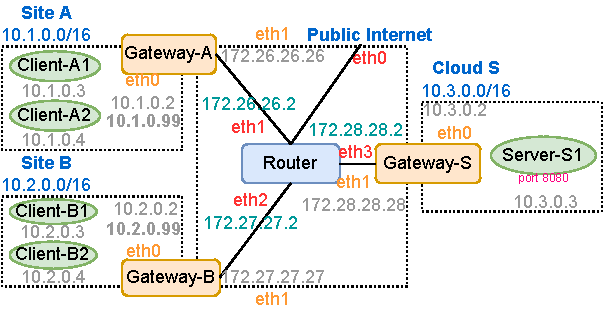
\includegraphics[width=1.1\textwidth]{figures/site-to-site.pdf}
    \caption{Site to Site}
    \label{fig:site2site}
  \end{center}
\end{figure}

A site-to-site VPN connects different network systems located at different sites together directly \cite{9022848}. In this case, the address space of site A, B and Cloud S should not overlap \cite{AKYILDIZ2023100695}.

Figure \ref{fig:site2site} shows the topology and corresponding address space under such circumstances.

\subsection{Gateway to Gateway}
\begin{figure}[t!]
  \begin{center}
    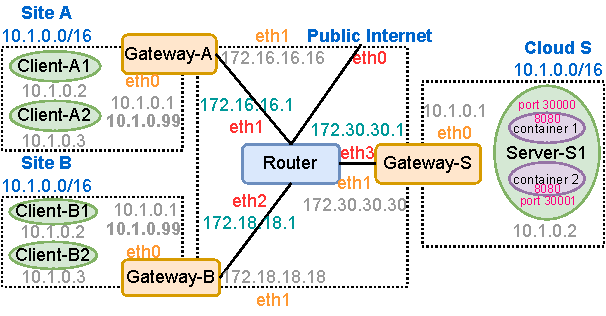
\includegraphics[width=1.1\textwidth]{figures/gateway-to-gateway.pdf}
    \caption{Gateway to Gateway}
    \label{fig:gateway2gateway}
  \end{center}
\end{figure}

A gateway-to-gateway VPN connects different gateways. The packages then get routed to different clients within the corresponding site according to the routing table of the gateway \cite{dulany2006performance}.

Figure \ref{fig:gateway2gateway} shows the topology and corresponding address space under such circumstances.

\subsection{Site to Site in IPv6}
\begin{figure}[t!]
  \begin{center}
    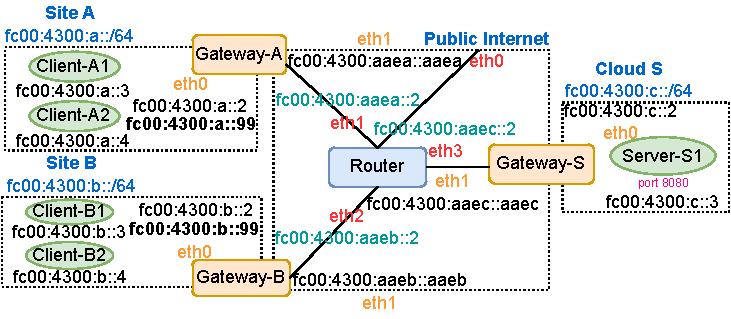
\includegraphics{figures/ipv6-site-to-site.pdf}
    \caption{Site to Site in IPv6}
    \label{fig:ipv6site2site}
  \end{center}
\end{figure}

Similar to Site to Site VPN in IPv4, but replace all the address space into IPv6.

Figure \ref{fig:ipv6site2site} shows the topology and corresponding address space under such circumstances.

%============================================================


\section{Implementation}

To manage the docker containers easily, we use Docker Compose to do the orchestration. Based on the figures above, we make each network component a separate container, assign the net\_admin capability to each container, and implement the network with the MacVLAN driver. To simulate the public Internet, we only connect the router to the docker default bridge network. Finally, we set up the routing and firewall, and configure the strongSwan IPSec correctly with certificates.

For routing, we use NAT Masquerade for the gateway interface so the local IP addresses can not be leaked outside their subnets. We bind the IP address 10.x.0.99 to the interface eth0 of gateway A and B.

We use strict firewall rules on the clients, as we assume there should be no need for the clients (IoT devices) to visit the Internet. We use iptables to set up firewall rules on gateway A and B for input and output. We accept IKE and ESP traffic (ESP traffic, port 500 and 4500 traffic in UDP) both from and to the cloud. Finally, we drop everything else, including the connection from and to the Internet.

There is also some difference between the two kinds of VPN setup:

\subsection{Site to Site}

Concerning routing, for gateway A and B, we redirect the traffic from the local address (10.1.0.99 and 10.2.0.99) of port 8080 to cloud server S1 of port 8080 with Destination NAT.

For the firewall, we also have to accept the post-routing traffic to the cloud server 10.3.0.3.

As there is no overlapping network address space within the site-to-site VPN, we can specify the IP address and subnet directly through Docker Compose. Also, we avoid using the IP address ending in ".1", as Docker does not allow us to assign that address to any container. These addresses are reserved for gateways or routers on a particular network (Even though we are simulating the Gateway and Router).

\subsection{Gateway to Gateway}

About routing, for gateway A and B, we redirect the traffic from the original local server address 10.x.0.99 of port 8080 to cloud gateway S of port 8080 with Destination NAT. For gateway S, we redirect the traffic from the client gateway A and B of port 8080 to corresponding ports (30000 and 30001) on the server s1 address.

There are overlapping network address spaces for gateway-to-gateway VPN. Suppose we specify the IP address and subnet directly through Docker Compose. In that case, there will be errors notifying us that "Pool overlaps with another one on this address space". Although technically, this should not be a problem, as we are creating a separate internal network without direct routing, Docker still forbids us.

We resolve the overlapping address space issue relatively hackingly, similar to IP address spoofing. When we do not specify the IP address of the network in Docker Compose, it will assign a random address from the docker address pool to the network interface. Now we can modify the IP address and subnet of the interface to our desired one, and no error will be thrown now.

In addition, for server S1, we use the Docker-in-Docker image to run docker containers inside the server S1 container. Running that image requires the container to be privileged according to the documentation \cite{docker}. As a result, in practice, we must ensure the software running in server S1 is benign and poses no risk to the host machine. Otherwise, it is generally not recommended to run the Docker-in-Docker image.

\subsection{Site to Site in IPv6}

Similar to Site to Site VPN in IPv4, just replace all the IPv4 address into IPv6 would complete the job.

%============================================================

\section{Evaluation}

We use Docker Engine 23.0.1 to run the containers and VirtualBox 7.0.6 to run the Virtual Machines.

The result shows that our container solution significantly reduces the fresh boot-up time\footnote{Include the base image building time} for the whole VPN system by nearly 90\%. The elapsed time for the containers orchestrated by Docker Compose to start is 75 seconds. In comparison, it takes 689 seconds for Virtual Machines to start with Vagrant.

The container solution dramatically reduces memory consumption when we start the VPN system and test the network communication as well. The containers started with Docker Compose take 278 MB of memory in total. In contrast, the Virtual Machines started with Vagrant take 4.5 GB of memory.

The shell script for making all the related routing and firewall configurations in Docker containers and VMs are identical, so it is easy to migrate configurations from the VMs to the docker containers. We can simultaneously start the site-to-site VPN setup and the gateway-to-gateway VPN setup in Docker without interfering.

We also verify that the command "ls /sys/devices/virtual/net -l" shows complete different results when executing from the host machine and inside the container.

Most importantly, our IPv4 setup can run in M1/M2 based Mac OS easily with docker desktop, while the VM ones fail to start.

%============================================================


\section{Conclusion}

This paper investigates the method to construct the testing environment of the VPN system through Docker containers. Containers are much more lightweight than virtual machines. As a mature virtualization technology already, containers can realize every functionality we require, just like virtual machines in our case, while increasing no security risk to the host machine that we run on top of.

We hope this paper can inspire researchers and engineers to migrate their testing environment related to network systems from VMs into containers.

%============================================================


% \section{Simple things first}

% In this section, we give some simple examples of Latex mark-up.
% Sec.~\ref{sec:emphasis} emphasizes important points and
% Sec.~\ref{sec:math} gives examples of math formulas.
% Finally, \ref{sec:list} demonstrates lists.


% %------------------------------------------------------------


% \subsection{Emphasizing text}
% \label{sec:emphasis}

% \textit{Italics} is a good way to emphasize printed text. However,
% \textbf{boldface} looks better when converted to HTML.

% Paragraphs are separated by an empty line in the Latex source code.
% Latex puts extra space between sentences, which you must suppress
% after a period that does not end a sentence, e.g.\ after this acronym.

% Cross-references to figures (Fig.~\ref{fig:mypicture1}), tables
% (Table~\ref{tab:mytable1}), other sections (Sec.~\ref{sec:math})
% are easy to create. 


% %------------------------------------------------------------


% \subsection{Mathematics}
% \label{sec:math}

% In the mathematics mode, you can have subscripts such as $K_{master}$
% and superscripts like $2^x$. Longer formulas may be put on a separate
% line:
% \[ \emptyset \in \emptyset \; \Rightarrow \; E \neq mc^2. \]

% You may also want to number the formulas like Eq.~(\ref{eqn:myequation1})
% below.
% \begin{equation}\label{eqn:myequation1}
% C = E_{K_{public}}(P) = P^e. \hspace{10mm}   P = D_{K_{private}}(C) = C^d.
% \end{equation}



% %------------------------------------------------------------


% \subsection{Make a list}
% \label{sec:list}

% Lists can have either bullets or numbers on them. 

% \begin{itemize}
% \item one item
% \item another item, which is an exceptionally long one for an item
%   and consequently continues on the next line.
% \end{itemize}

% Lists can have several levels. Item~\ref{kukkuu} below contains
% another list.
% \begin{enumerate}
% \item the fist item \label{kukkuu}
%   \begin{enumerate}
%   \item the first subitem 
%   \item the second subitem
%   \end{enumerate}
% \item the second item
% \end{enumerate}


% %============================================================


% \section{More complex stuff}

% This section provides examples of more complex things.


% %------------------------------------------------------------


% \subsection{Data served on a table}


% Table~\ref{tab:mytable1} presents some data in tabular form. 

% \begin{table}[t!]
%   \begin{center}
%     \begin{tabular}{|l|lr|}
%     \hline
%     Protocol & Year &  RFC \\
%     \hline
%     TCP      & 1981 &  793 \\
%     ISAKMP   & 1998 & 2408 \\
%     Photuris & 1999 & 2522 \\
%     \hline
%     \end{tabular}
%     \caption{A table with some protocols}
%     \label{tab:mytable1}
%   \end{center}
% \end{table}


% %------------------------------------------------------------


% \subsection{Adding references}
% \label{sec:references}

% Do not forget to give pointers to the literature. If you are listing
% stuff related to your topic, you can give several references once
% \cite{Com00,HTS03,Nik99}. However, usually you should give only one, for example the standard describing the stuff \cite{RFC2408} and if you want to directly use someone else's words, use both quotation marks and refer to the source, for example that ``the developer does not need to know all about the framework to develop a working implementation'' \cite{Suo98}. Remember also to mark references to your pictures if they are not created by your own mind!

% If you plan to write with Latex regularly, create your own BibTeX
% database and use BibTeX to typeset the bibliographies automatically.
% In the long run, it will save you a lot of time and effort compared to
% compiling reference lists by hand.


% %------------------------------------------------------------


% \subsection{Embedded pictures}
% \label{sec:pictures}

% Fig.~\ref{fig:mypicture1} is an embedded picture. The supported formats for pictures
% depend on the actual LaTeX command used. For instance, regular \LaTeX supports
% pictures in EPS (Embedded PostScript) format, while pdf\LaTeX supports PDF (Portable
% Document Format), PNG (Portable Network Graphics) and JPEG (Joint Photographic Experts
% Group). It is recommended to use either EPS or PDF for diagrams as well as for any picture
% which includes vector images.

% \begin{figure}[t!]
%   \begin{center}
%     % Note how the file extension has been removed from the filename below
%     % so that the LaTeX command can automatically pick any supported file format
%     \includegraphics[width=.5\textwidth]{figures/sample}
%     \caption{An embedded picture}
%     \label{fig:mypicture1}
%   \end{center}
% \end{figure}


% %============================================================


% \section{Yet another section title}

% To be added.


%============================================================


\bibliographystyle{plain}
\bibliography{cs-seminar}

\end{document}
